\documentclass[11pt]{article}

\usepackage[margin=0.7in]{geometry}
\usepackage{graphicx}
\usepackage{booktabs}
\usepackage{hyperref}
\usepackage{amsmath}
\usepackage{placeins}
\usepackage{enumitem}
\usepackage{titlesec}
\usepackage{array}
\usepackage{tabularx}

\hypersetup{colorlinks=true, linkcolor=blue, urlcolor=blue, citecolor=blue}
\renewcommand{\arraystretch}{1.25}

\setlength{\textfloatsep}{8pt plus 1pt minus 2pt}
\setlength{\floatsep}{6pt plus 1pt minus 1pt}
\setlength{\intextsep}{6pt plus 1pt minus 1pt}
\renewcommand{\topfraction}{0.9}
\renewcommand{\bottomfraction}{0.8}
\renewcommand{\textfraction}{0.07}
\setcounter{topnumber}{4}
\setcounter{bottomnumber}{4}
\setcounter{totalnumber}{6}
\raggedbottom

\titleformat{\section}{\normalfont\large\bfseries}{\thesection}{0.6em}{}
\titleformat{\subsection}{\normalfont\bfseries}{\thesubsection}{0.6em}{}
\titlespacing*{\section}{0pt}{1.4em}{0.6em}
\titlespacing*{\subsection}{0pt}{1.0em}{0.4em}

\title{\Large Opinion Network Formation: How This Class's Views on\\
Technology, Education, Society, and the Environment Fit Together}
\author{}
\date{}

\begin{document}
\maketitle
\vspace{-3.5em}

\noindent
\begin{tabular}{@{}ll}
\textbf{Team Name:} & Asstra \\
\textbf{Team Members:} & Shreyas Deb, Abhishek, Sampath \\
\textbf{Repository:} & \url{https://github.com/shrey715/dpcn-opinion_network-asstra}
\end{tabular}

\vspace{0.8em}
\hrule
\vspace{0.4em}

\section{Dataset Documentation}

The survey collected 96 responses across 60 Likert-scale statements, split into four blocks:
Technology (T01--T15), Education (E01--E15), Society and Ethics (S01--S15), and Environment and Values
(V01--V15). We mapped Strongly Disagree through Strongly Agree to the integers 1 through 5. A few
respondents answered "No Comments" on individual items instead of picking a point on the scale; we
coded those as missing rather than forcing them to the midpoint, since a shrug isn't the same as
"Neutral."

\paragraph{Respondent filtering.} Five people left the whole survey blank and got dropped outright. Six
more stopped partway through, and not randomly: each answered items $1, \dots, N$ in order and then
left everything after that blank. That looks like fatigue, not scattered skipping. A further 17 people
finished the survey but marked "No Comments" on one to four items scattered through it, so those got
coded as missing too. That's the full breakdown of all 96: 5 blank, 6 partial with a clean cutoff, 17
partial with scattered gaps, and 68 who answered everything. Every analysis that needs a complete
numeric matrix uses only those 68, so the partial responses can't skew a correlation.

\paragraph{Descriptive summary.} Before building any network, it's worth checking what the class
agreed on and what it fought about, since that shapes what a correlation network can even find. The
numbers below come from the 91 non-blank respondents (all 96 minus the 5 blank surveys), not the 68
used everywhere from Section~2 on; the two samples give slightly different numbers, and these are the
91-respondent ones. Environment has the highest mean (4.39 out of 5) and the tightest spread of any
block (mean per-item standard deviation 0.72): pretty much nobody disagrees that companies should
answer for their environmental impact. Education has the lowest mean (3.91), and its item E03 ("class
attendance should be compulsory") is the single most contested statement in the whole survey, mean
2.06, standard deviation 1.12. By spread rather than mean, though, Technology is actually the most
divided block (0.92), just ahead of Education (0.89), so Education has the lowest mean but not the
widest spread. This consensus-versus-conflict split shows up again, more sharply, once we look at the
data as a network instead of a table of averages (Section~4), though Section~4 also shows part of that
network-level split comes from a general agreement factor rather than topic content alone.

\section{Pipeline Followed}

We built four networks from the same cleaned data, each aimed at a different question about how the
class's opinions fit together. In every case an edge, whether between two statements or two
respondents, means their answers move together across the sample: a Pearson correlation, weighted by
its strength. Table~\ref{tab:networks} summarizes all four before we walk through each one.

\begin{table}[htbp]
    \centering
    \caption{The four network constructions at a glance.}
    \label{tab:networks}
    \footnotesize
    \begin{tabularx}{\textwidth}{@{}lXXX@{}}
        \toprule
        Network & Nodes & Edge rule & Validation \\
        \midrule
        Idea & 60 statements & $|r| \geq 0.15$, weighted & permutation null ($B{=}1000$) \\
        Extension 1 & 60 statements & unsigned, $\tau \in [0.10, 0.45]$ & Erdos-Renyi null ($B{=}200$) \\
        Extension 2 & 68 respondents & 5-NN, profile correlation & leave-one-item-out + bootstrap \\
        Extension 3 & 60 statements (4 blocks) & within-block $|r|$, unthresholded & permutation null ($B{=}200$, per block) \\
        \bottomrule
    \end{tabularx}
\end{table}

\subsection{Idea: the statement co-endorsement network}

The 60 statements are the nodes. Two statements get an edge if the absolute Pearson correlation
between their answers, across the 68 complete respondents, is at least 0.15, weighted by that
correlation. That gives 907 edges on 60 nodes, a deliberately dense graph. Cutting down to a sparse
top-$N\%$ graph would just bake in an arbitrary cutoff; keeping the full graph means centrality
reflects the whole correlation structure instead of whatever a cutoff happened to keep. On this graph
we ran eigenvector centrality and PageRank, which both find statements near the core of the belief
system, plus betweenness centrality for statements that bridge otherwise separate clusters. We also
ran $k$-core decomposition on a stricter $|r| \geq 0.30$ version to find a backbone: the subgraph left
after repeatedly stripping out any node connected to fewer than $k$ others in it.

We checked significance with a permutation test: shuffle each of the 60 item columns independently
across respondents, 1000 times, which wipes out any real correlation but keeps each item's own
response distribution intact. Then we compare the real statistic to that null distribution. Raw
Pearson correlation is also sensitive to how agreeable a respondent is overall, so we separately
reran the whole thing on a version of the data where each respondent's own mean response is
subtracted out first. Both readings are discussed together in Section~4.1.

\subsection{Extension 1: structure and sensitivity of the statement network}

This part asks four questions about the statement network's structure, all on the same 60 nodes.
\textbf{1a} checks whether the graph at $|r| \geq 0.20$ (647 edges: 620 positive, 27 negative) is more
triangle-dense than a random graph of the same size and density would be. We compared the observed
triangle count to an Erdos-Renyi graph $G(60, \hat p)$, both through the closed form
$\binom{60}{3}\hat p^3$ and through 200 simulated draws. \textbf{1b} pulls the 27 negative edges out
and looks at them as their own subgraph: degree, connected components, and whether any triangles form
among purely negative relationships. \textbf{1c} sweeps the edge threshold $\tau$ from 0.10 to 0.45
and tracks edge count, giant-component size, and isolated-node count against their own nulls (a
permutation null for the first two, the Erdos-Renyi formula $n(1-\hat p)^{n-1}$ for isolated nodes),
plus the Technology-versus-rest degree gap at every threshold. \textbf{1d} builds a structural table,
density, mean degree, degree variance, components, diameter, average path length, clustering, and
degree-weighted average-neighbor-degree at $|r| \geq 0.15, 0.20, 0.30$, against the matching
Erdos-Renyi predictions, plus the degree distribution at $|r| \geq 0.30$ against a
Binomial$(n{-}1, p)$ null. 1d also answers a question the Idea section leaves open: why 0.15? A
permutation null tells us what fraction of edges at each threshold is there by chance alone.

\subsection{Extension 2: the respondent similarity network}

Here the 68 respondents are the nodes, each linked to its five nearest neighbors by profile
correlation. We used this network to predict every one of the $68 \times 60 = 4080$ (respondent, item)
answers from a respondent's neighbors, and compared the error to a global item-mean baseline.
Similarity for predicting a given item is recomputed with that item's own column dropped first, so a
respondent's real answer never sneaks into the neighbor selection used to predict it. Since the 4080
cells come from only 68 people, we used a respondent-level bootstrap instead of a cell-level test that
would wrongly treat correlated cells as independent. We also draw the network itself as a directed
graph (Figure~\ref{fig:imputation}, since each respondent points to five others but isn't necessarily
pointed back at by the same five) along with its in-degree distribution.

\subsection{Extension 3: per-block network density}

The 60 statements split into four blocks, T, E, S, V, each treated as its own induced subgraph of the
full statement-correlation graph, with no edges across blocks. Each block's weighted link density is
the mean of $|r|$ over every pair inside it, straight off the correlation matrix. We test that density
against a permutation null built the same way as Section~2.1's, run separately per block, and check it
against the closed-form expected value of $|r|$ for two independent 68-observation vectors. Like the
Idea network, we reran this on a row-centered correlation matrix as a robustness check (Section~4.4).

\section{Analysis and Visualizations}

The figures and tables below cover all four networks and their significance tests, in the same order
as Section 2. Section 4 walks through what each one means.

\begin{figure}[htbp]
    \centering
    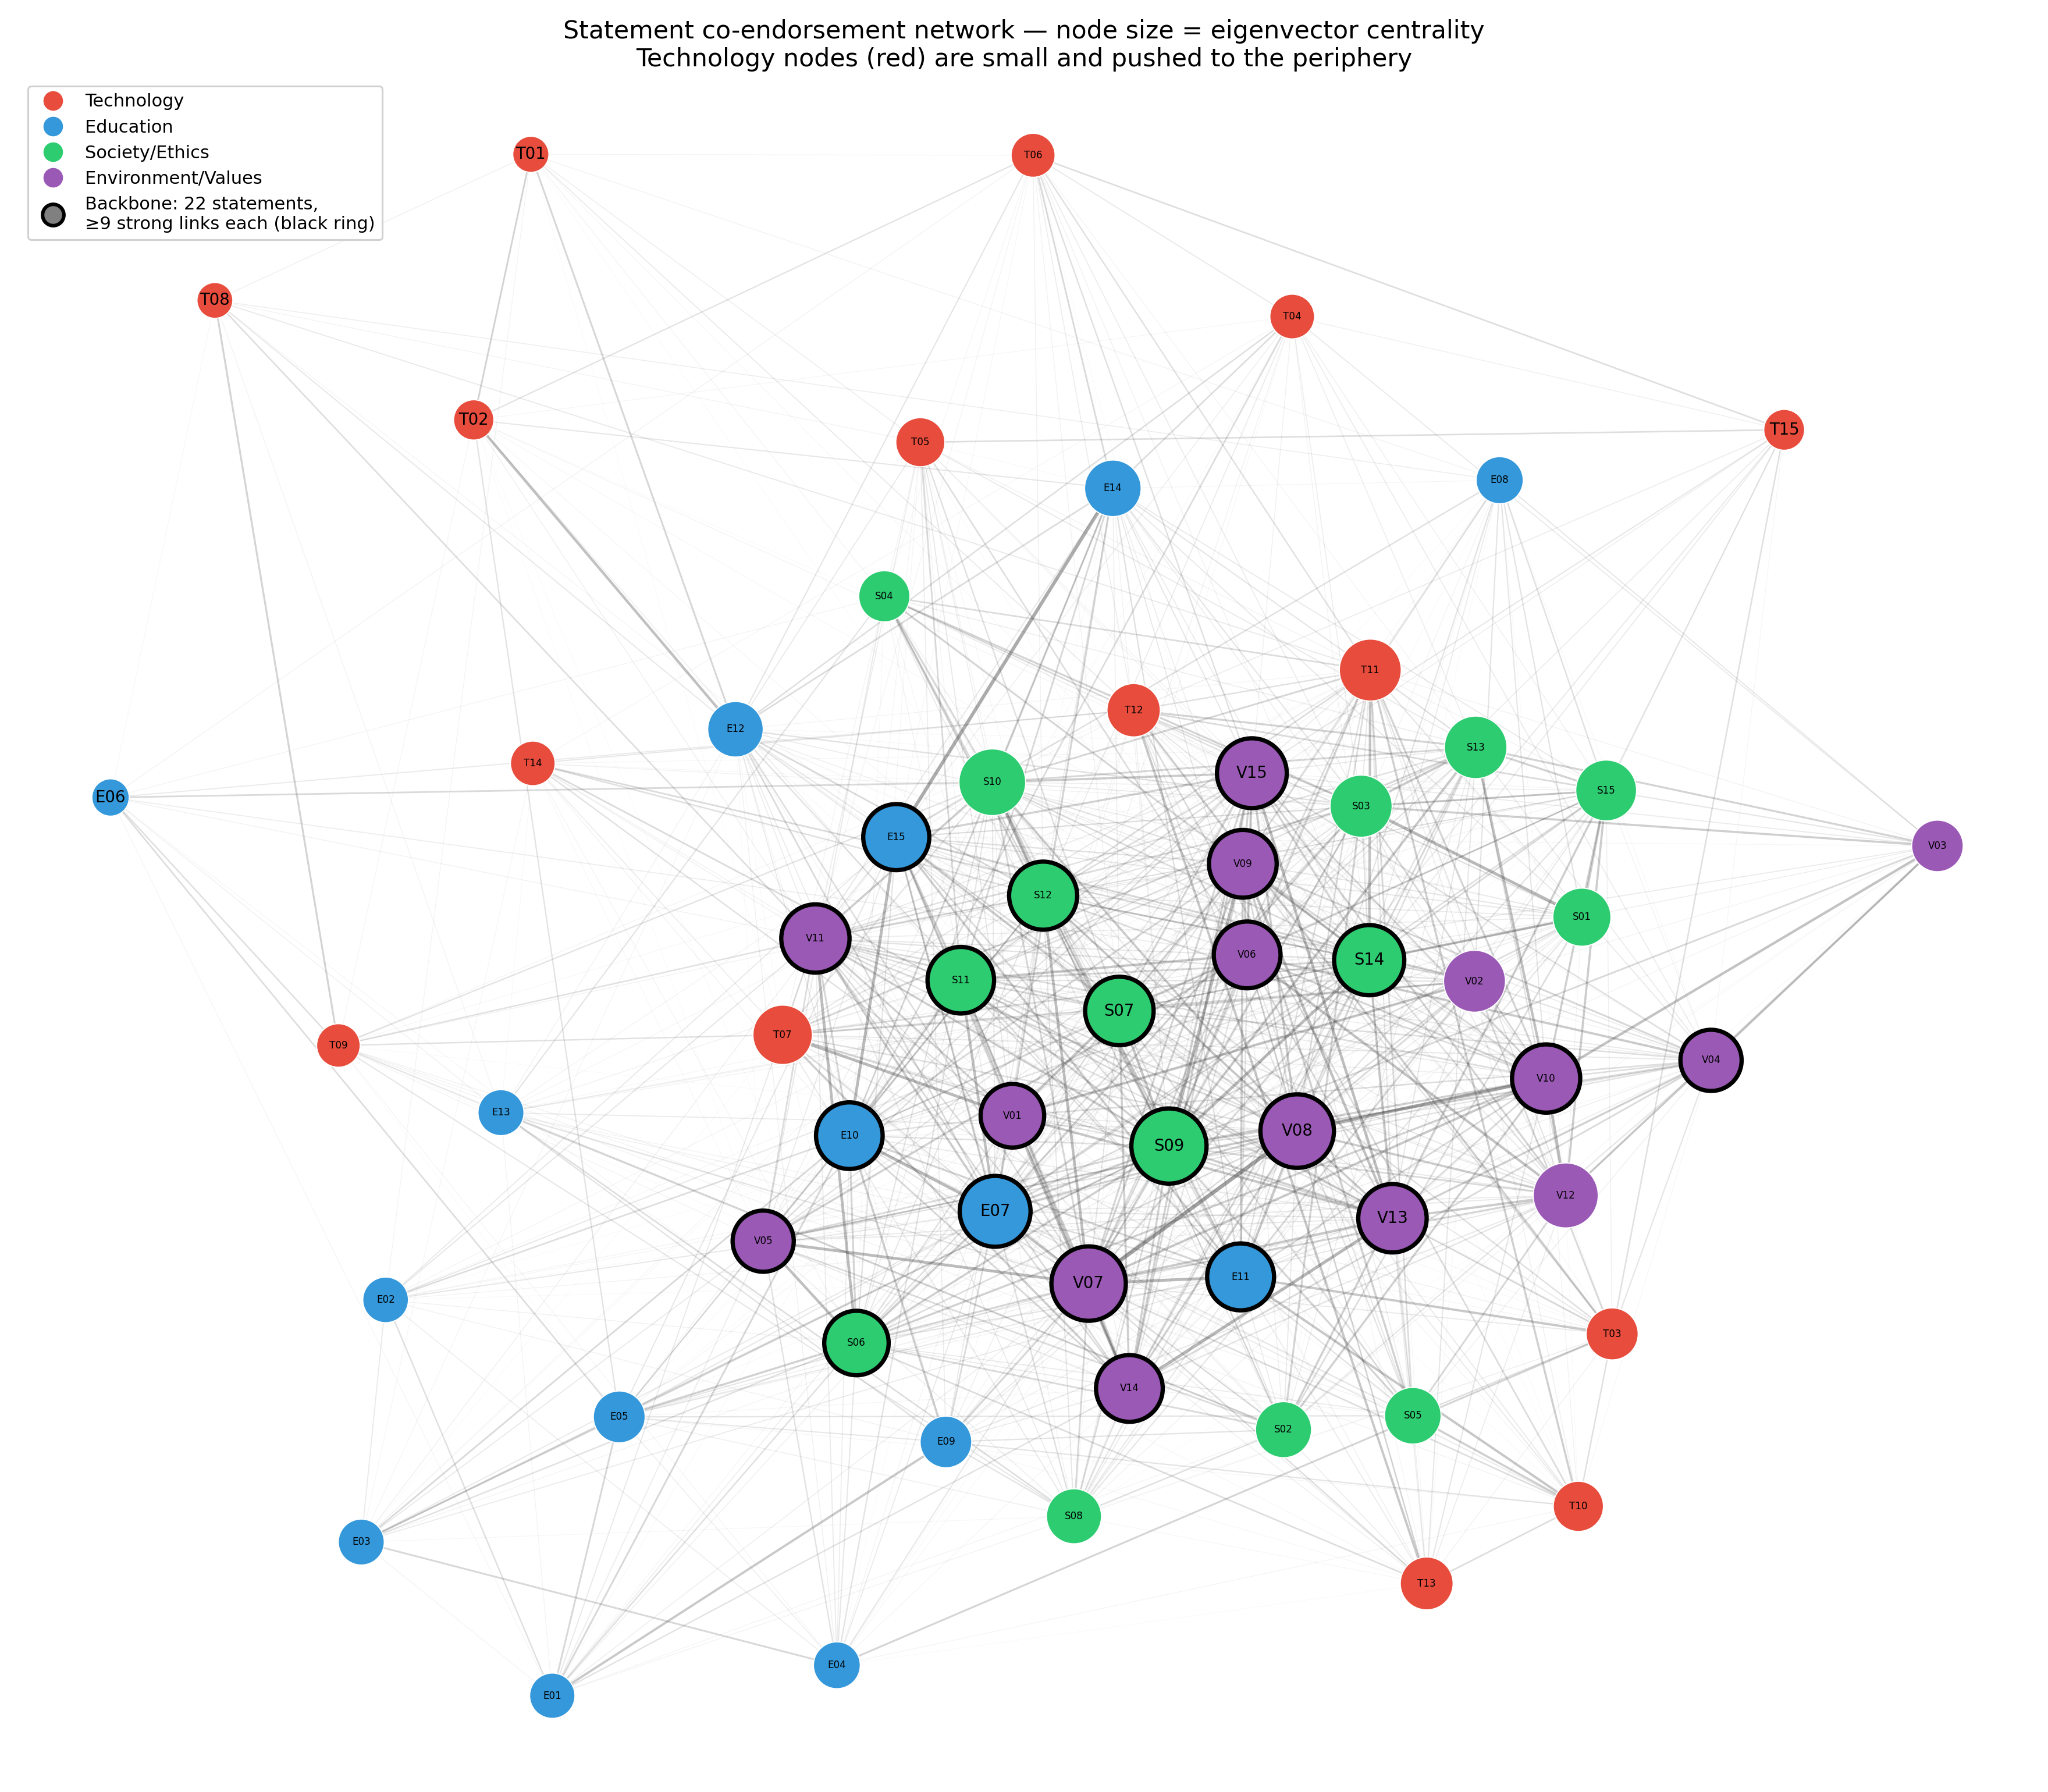
\includegraphics[width=0.85\textwidth]{../outputs/network_graph.png}
    \caption{The statement co-endorsement network. Node size is eigenvector centrality, color is
    the T/E/S/V block, a black ring marks the 22-statement backbone. Technology nodes are small
    and sit toward the edge.}
    \label{fig:network}
\end{figure}

\begin{figure}[htbp]
    \centering
    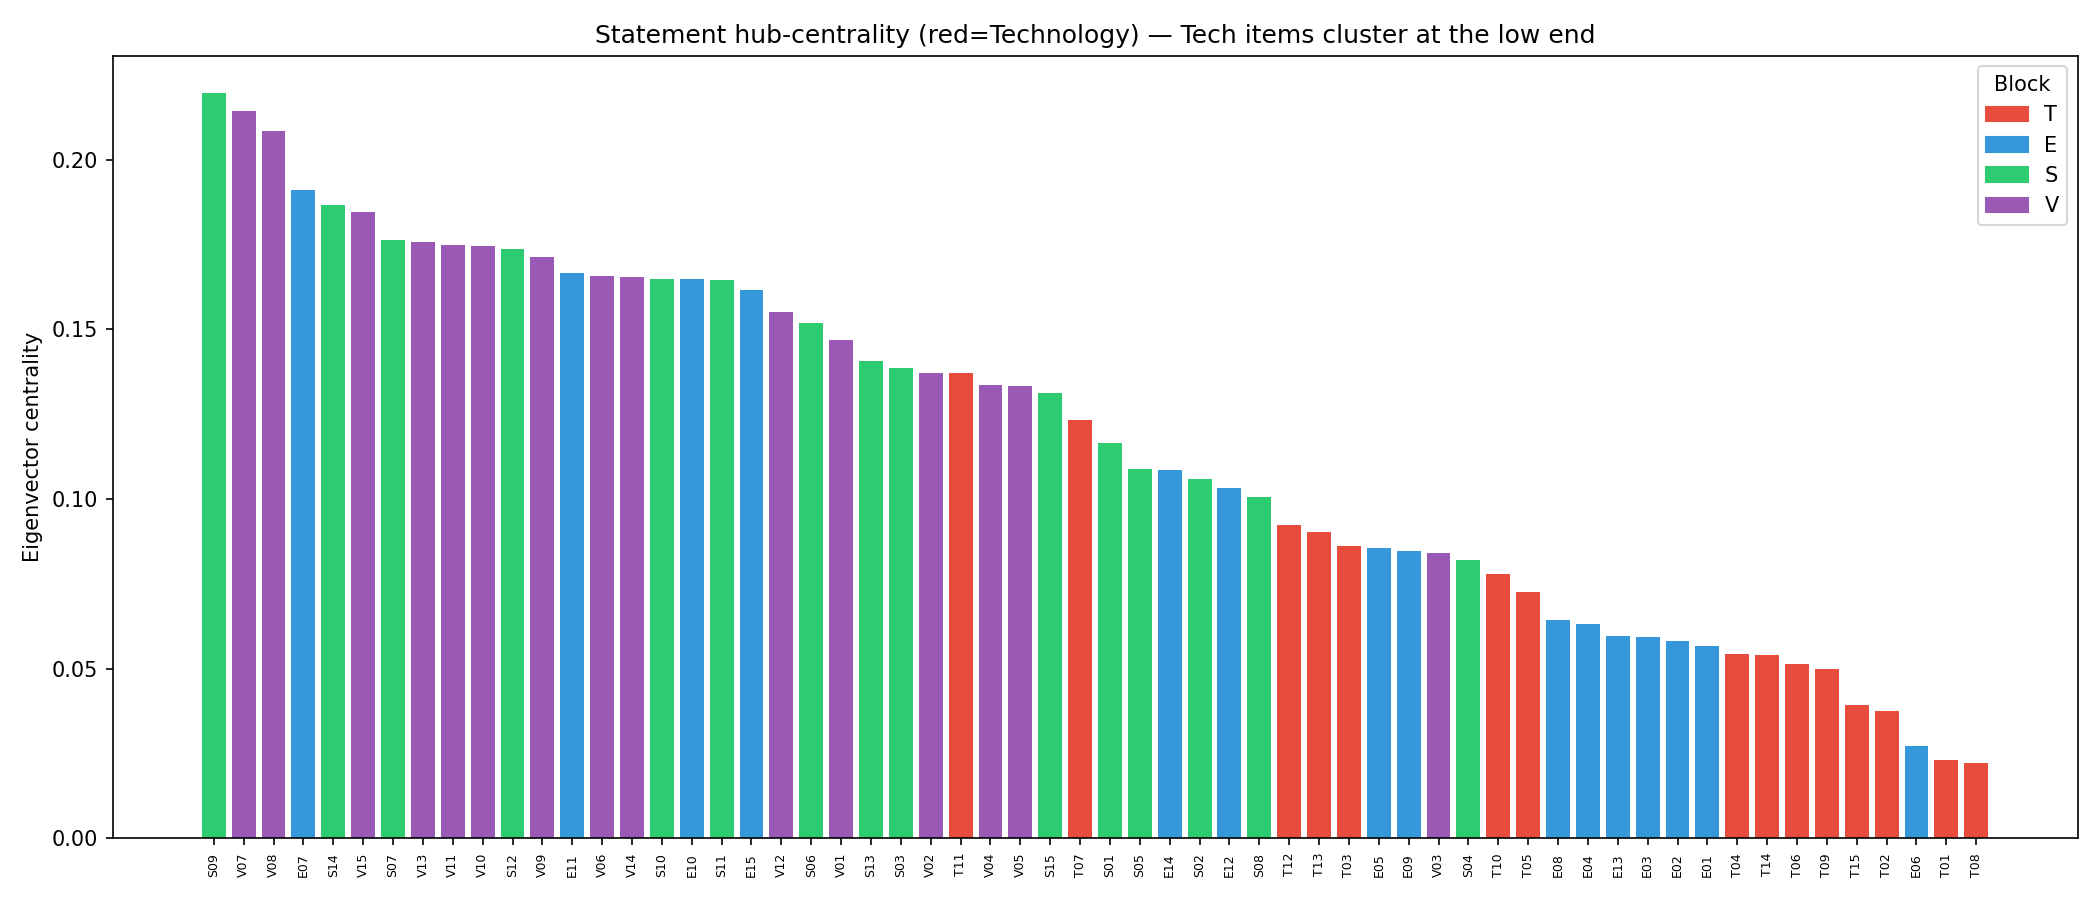
\includegraphics[width=0.85\textwidth]{../outputs/centrality_by_statement.png}
    \caption{Eigenvector centrality for all 60 statements, sorted and colored by block.
    Technology clusters at the low end.}
    \label{fig:centrality}
\end{figure}

\begin{figure}[htbp]
    \centering
    \begin{minipage}{0.48\textwidth}
        \centering
        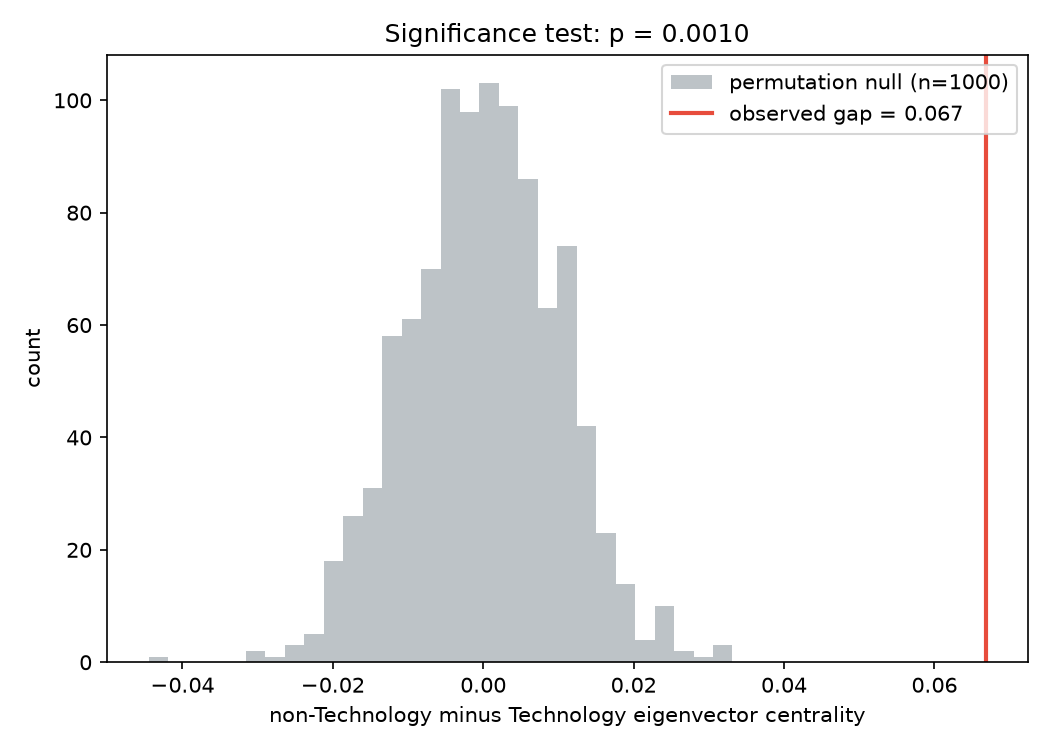
\includegraphics[width=\textwidth]{../outputs/significance_test.png}
        \caption{Permutation test for the centrality gap: the real value (red line) against 1000
        reshuffled versions of the data (gray bars).}
        \label{fig:sig-idea}
    \end{minipage}
    \hfill
    \begin{minipage}{0.48\textwidth}
        \centering
        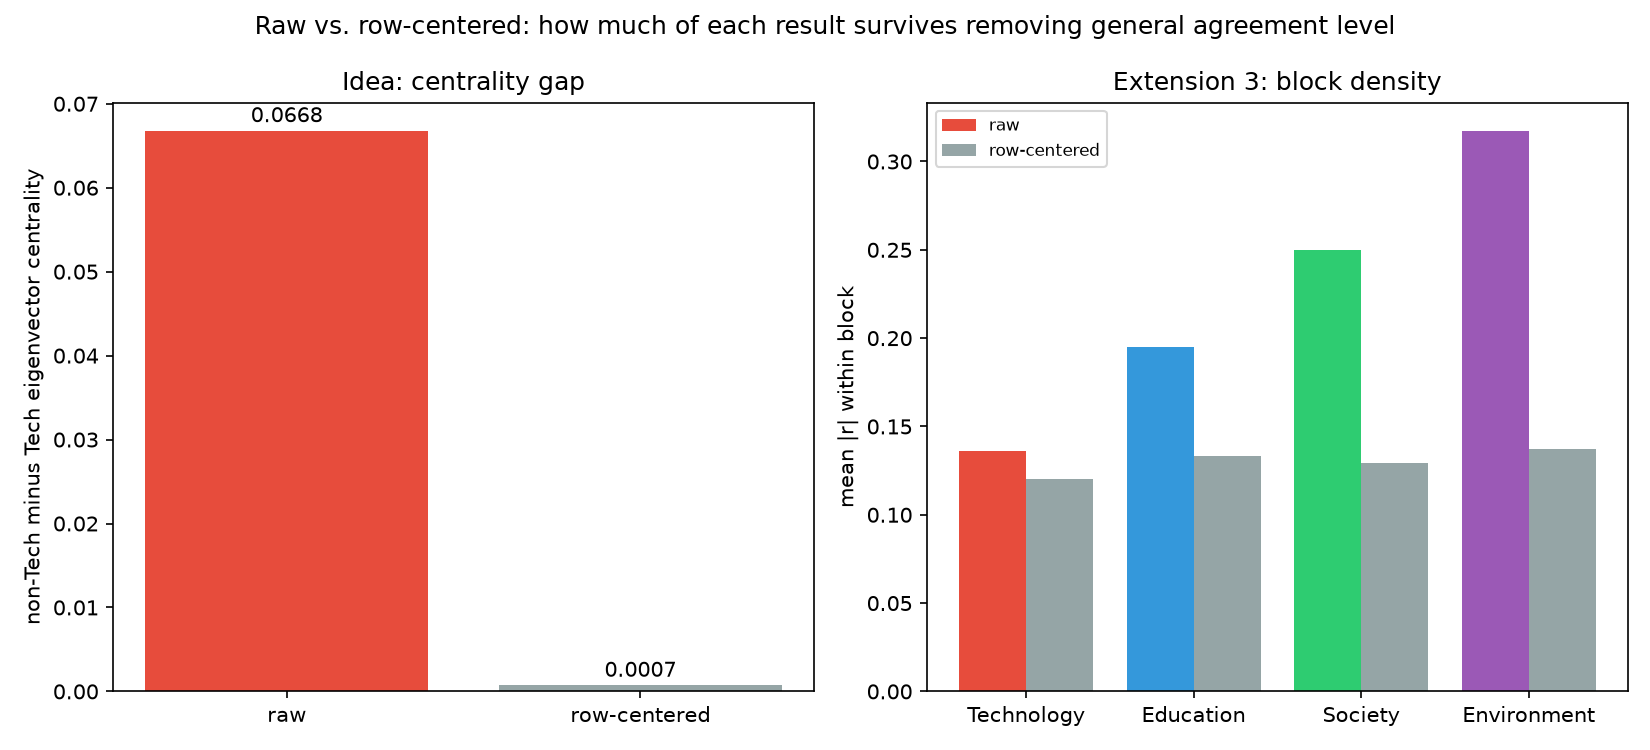
\includegraphics[width=\textwidth]{../outputs/raw_vs_rowcentered.png}
        \caption{Raw versus row-centered: the centrality gap and the four block densities, before and
        after subtracting each respondent's general agreement level. Both shrink a lot.}
        \label{fig:rowcentered}
    \end{minipage}
\end{figure}

\begin{figure}[htbp]
    \centering
    \begin{minipage}{0.48\textwidth}
        \centering
        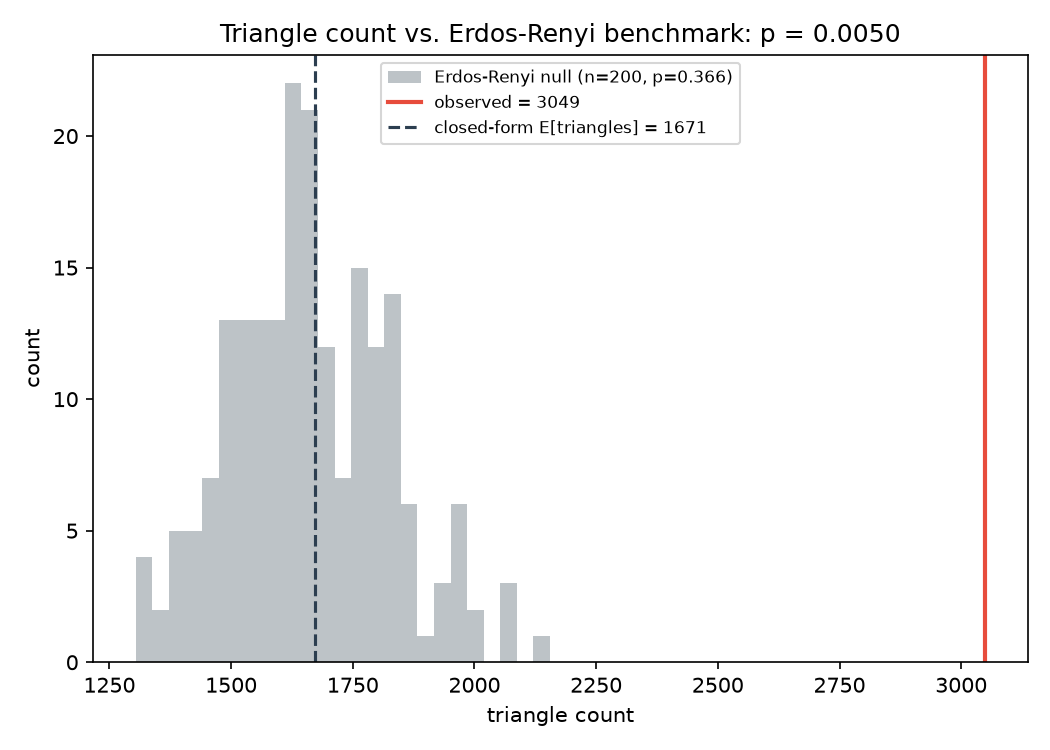
\includegraphics[width=\textwidth]{../outputs/triangle_significance.png}
        \caption{1a: observed triangle count in the 647-edge graph (red line) against 200 simulated
        Erdos-Renyi graphs of the same size and density (gray bars).}
        \label{fig:triangle}
    \end{minipage}
    \hfill
    \begin{minipage}{0.48\textwidth}
        \centering
        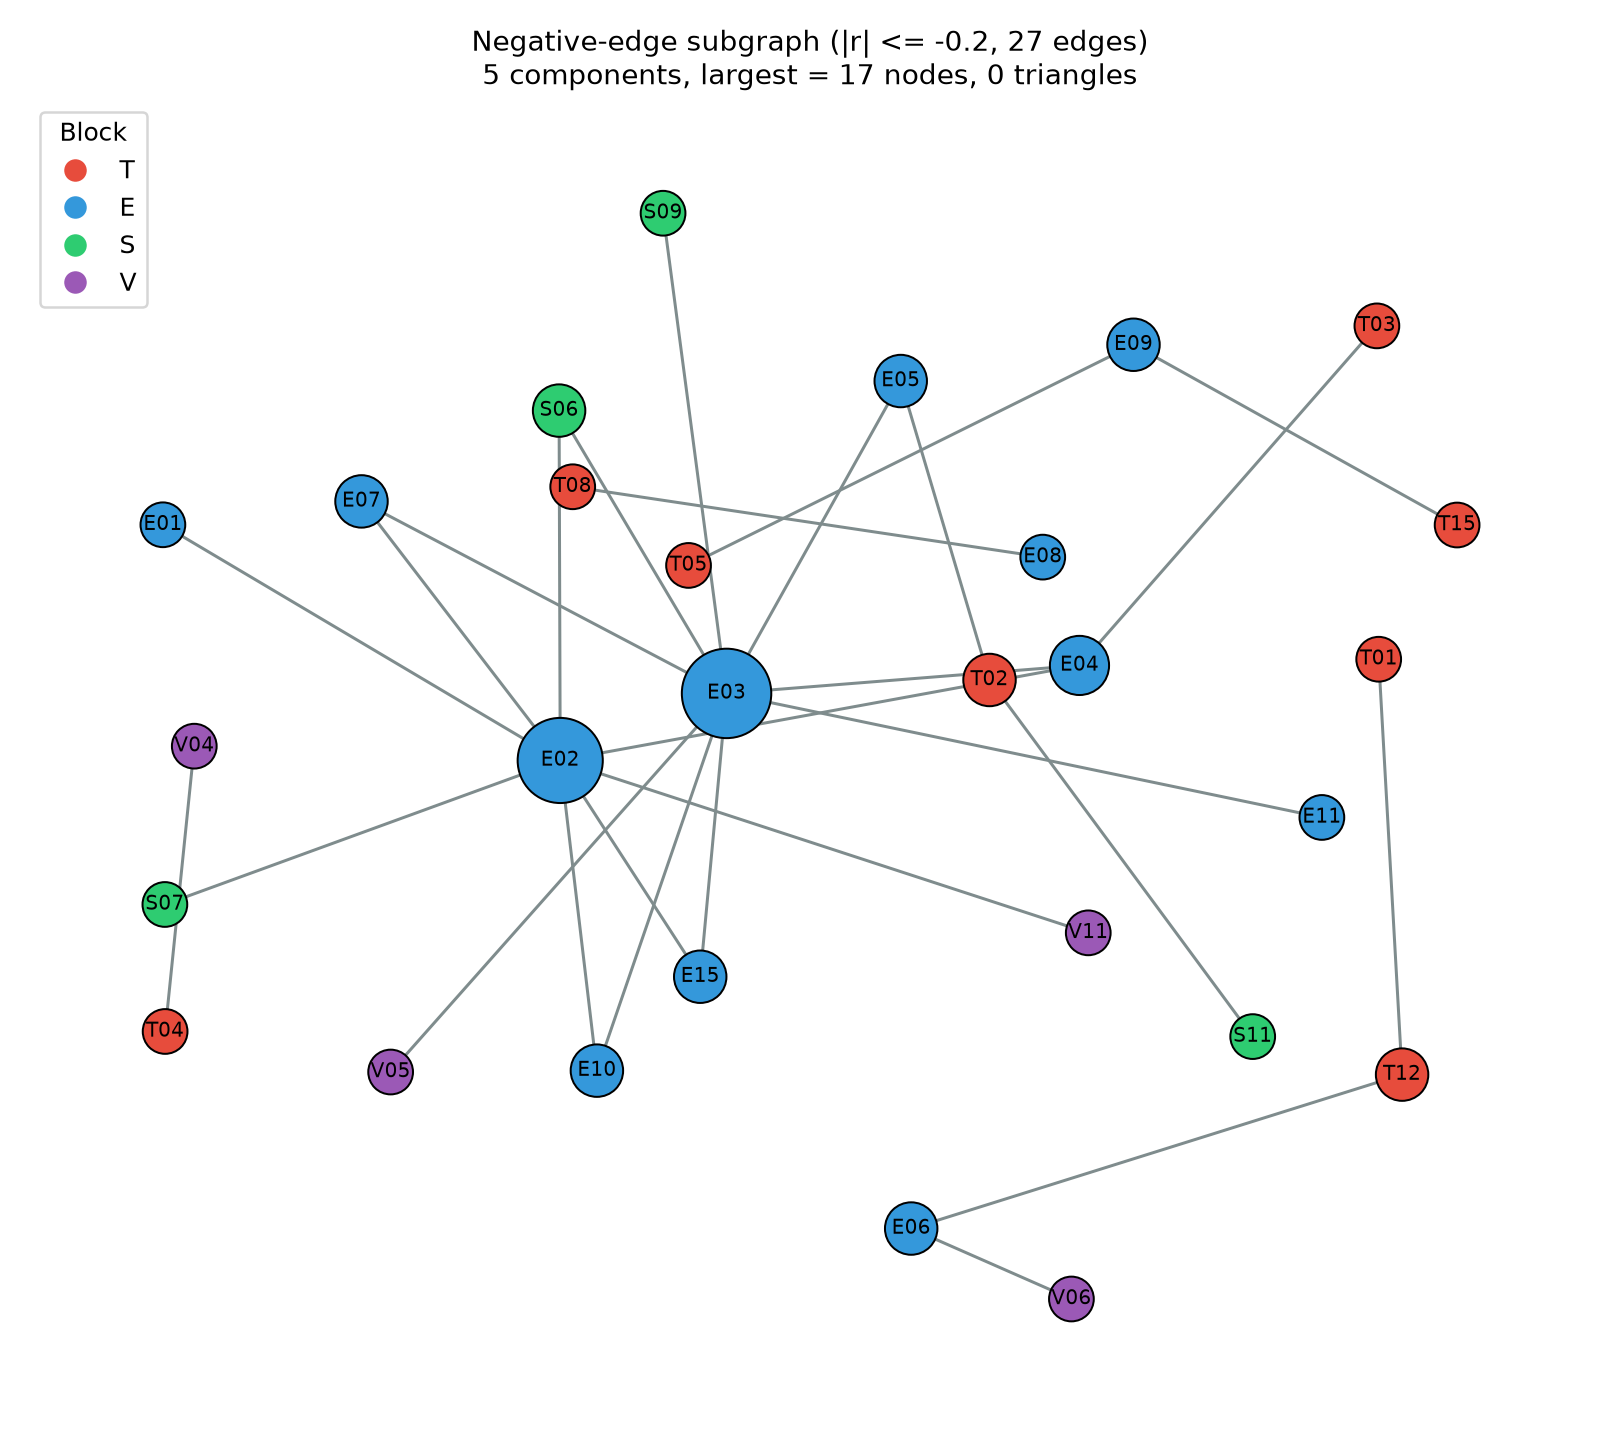
\includegraphics[width=\textwidth]{../outputs/negative_edge_subgraph.png}
        \caption{1b: the 27 negative edges as their own subgraph. Node size is degree within this
        subgraph; E03 and E02 (both Education) anchor the biggest component.}
        \label{fig:negedge}
    \end{minipage}
\end{figure}

\begin{table}[htbp]
    \centering
    \caption{1c: threshold sweep over $\tau \in [0.10, 0.45]$. Edges and giant-component size are
    shown observed vs.\ permutation null; isolated nodes are observed vs.\ the Erdos-Renyi prediction
    $n(1-\hat p)^{n-1}$; the last column is the Technology-versus-rest mean-degree gap.}
    \label{tab:sweep}
    \footnotesize
    \begin{tabular*}{\textwidth}{@{\extracolsep{\fill}}cccccccc@{}}
        \toprule
        $\tau$ & edges (obs) & edges (null) & giant (obs) & giant (null) & isolated (obs) & isolated (ER) & Tech gap \\
        \midrule
        0.100 & 1172 & 734.1 & 60 & 60.0 & 0 & 0.00 & 9.956 \\
        0.125 & 1029 & 554.9 & 60 & 60.0 & 0 & 0.00 & 11.600 \\
        0.150 & 907  & 399.1 & 60 & 60.0 & 0 & 0.00 & 11.689 \\
        0.175 & 783  & 272.6 & 60 & 60.0 & 0 & 0.00 & 11.511 \\
        0.200 & 647  & 177.5 & 60 & 59.9 & 0 & 0.00 & 11.956 \\
        0.225 & 565  & 115.2 & 60 & 58.8 & 0 & 0.00 & 11.244 \\
        0.250 & 457  & 68.5  & 60 & 51.0 & 0 & 0.00 & 9.822  \\
        0.275 & 368  & 37.5  & 60 & 21.6 & 0 & 0.00 & 8.089  \\
        0.300 & 304  & 23.6  & 60 & 9.6  & 0 & 0.00 & 6.844  \\
        0.325 & 233  & 11.8  & 56 & 3.8  & 2 & 0.01 & 6.178  \\
        0.350 & 171  & 6.4   & 47 & 3.1  & 8 & 0.15 & 5.289  \\
        0.375 & 125  & 3.7   & 44 & 2.5  & 12 & 0.80 & 3.956 \\
        0.400 & 95   & 1.6   & 42 & 2.0  & 16 & 2.32 & 3.067 \\
        0.425 & 59   & 0.6   & 35 & 1.4  & 19 & 8.12 & 2.000 \\
        0.450 & 41   & 0.2   & 33 & 1.2  & 21 & 15.05 & 1.200 \\
        \bottomrule
    \end{tabular*}
\end{table}

\begin{table}[htbp]
    \centering
    \caption{1d: structural stats at three thresholds, observed value with the Erdos-Renyi prediction
    in parentheses.}
    \label{tab:structural}
    \footnotesize
    \begin{tabular*}{\textwidth}{@{\extracolsep{\fill}}cccccccc@{}}
        \toprule
        $\tau$ & edges & density & $\langle k \rangle$ & diameter & Var($k$) & $\langle L \rangle$ & $C$ / $\langle k_{nn}\rangle$ \\
        \midrule
        0.15 & 907 & 0.512 & 30.2 & 2 & 94.3 (15.0) & 1.49 (1.20) & 0.64 (0.51) / 33.4 (30.7) \\
        0.20 & 647 & 0.366 & 21.6 & 3 & 95.0 (13.9) & 1.67 (1.33) & 0.57 (0.37) / 26.0 (22.2) \\
        0.30 & 304 & 0.172 & 10.1 & 5 & 45.2 (8.5)  & 2.21 (1.77) & 0.45 (0.17) / 14.6 (11.0) \\
        \bottomrule
    \end{tabular*}
\end{table}

\begin{table}[htbp]
    \centering
    \caption{One headline statistic per analysis, tested against its own null.}
    \label{tab:headline}
    \footnotesize
    \begin{tabularx}{\textwidth}{@{}lXXX@{}}
        \toprule
        Analysis & Statistic & Observed & Test \\
        \midrule
        Idea (raw) & Eigenvector centrality gap, non-Tech $-$ Tech & 0.0668 & $p=0.0010$ ($B{=}1000$) \\
        Idea (row-centered) & Same statistic, agreement level removed & 0.0007 & near null, see \S4.1 \\
        Ext.\ 1a & Triangle count, 647-edge graph & 3049 & $p=0.0050$ vs.\ ER null \\
        Ext.\ 1b & Negative-edge subgraph & hub-and-spoke on E03/E02, 0 triangles & descriptive \\
        Ext.\ 1d & Clustering at $\tau=0.30$, obs vs.\ ER & 0.45 vs.\ 0.17 & Table~\ref{tab:structural} \\
        Ext.\ 2 & Network $k$-NN MAE / baseline (4080 cells) & 0.645 / 0.662 & 95\% CI $[-0.010, 0.042]$ \\
        Ext.\ 3 & Within-block mean $|r|$, T/E/S/V & 0.136/0.195/0.250/0.318 & $p=0.0050$ (all four) \\
        \bottomrule
    \end{tabularx}
\end{table}

\begin{figure}[htbp]
    \centering
    \begin{minipage}{0.4\textwidth}
        \centering
        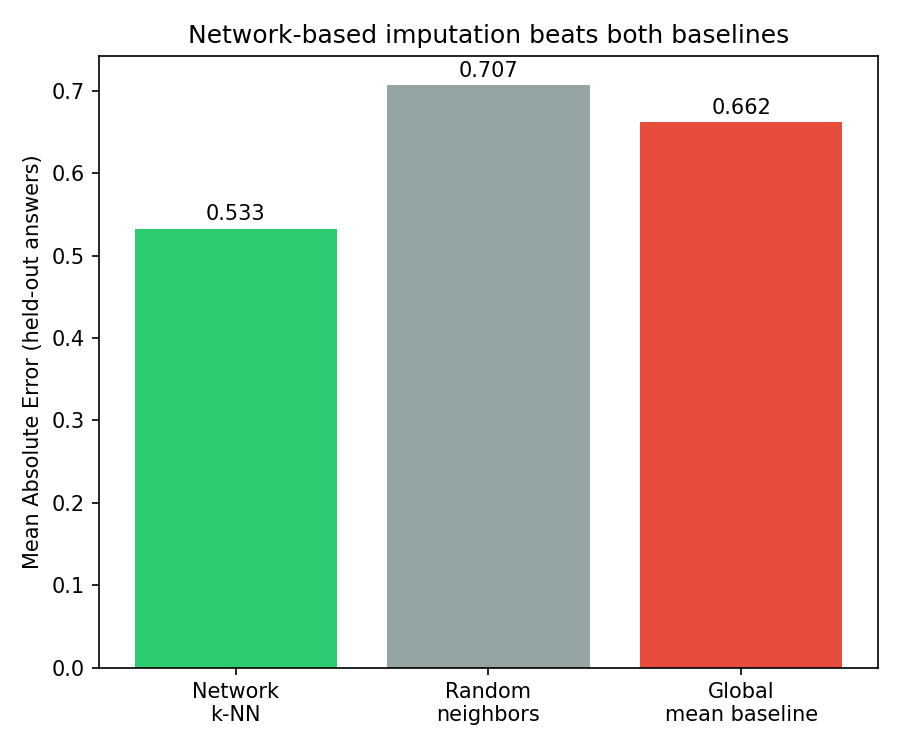
\includegraphics[width=\textwidth]{../outputs/imputation_mae.png}\\[2pt]
        \small\textit{MAE over all 4080 cells.}
    \end{minipage}
    \hfill
    \begin{minipage}{0.4\textwidth}
        \centering
        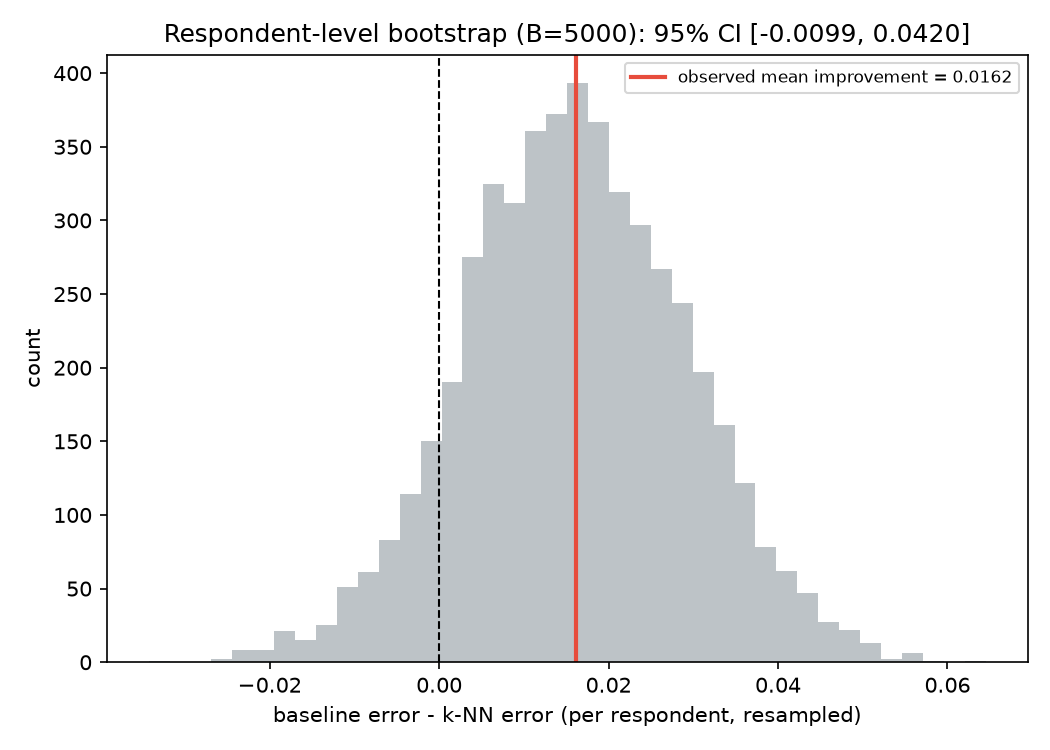
\includegraphics[width=\textwidth]{../outputs/imputation_bootstrap.png}\\[2pt]
        \small\textit{Respondent-level bootstrap; the 95\% CI includes zero.}
    \end{minipage}

    \vspace{0.5em}
    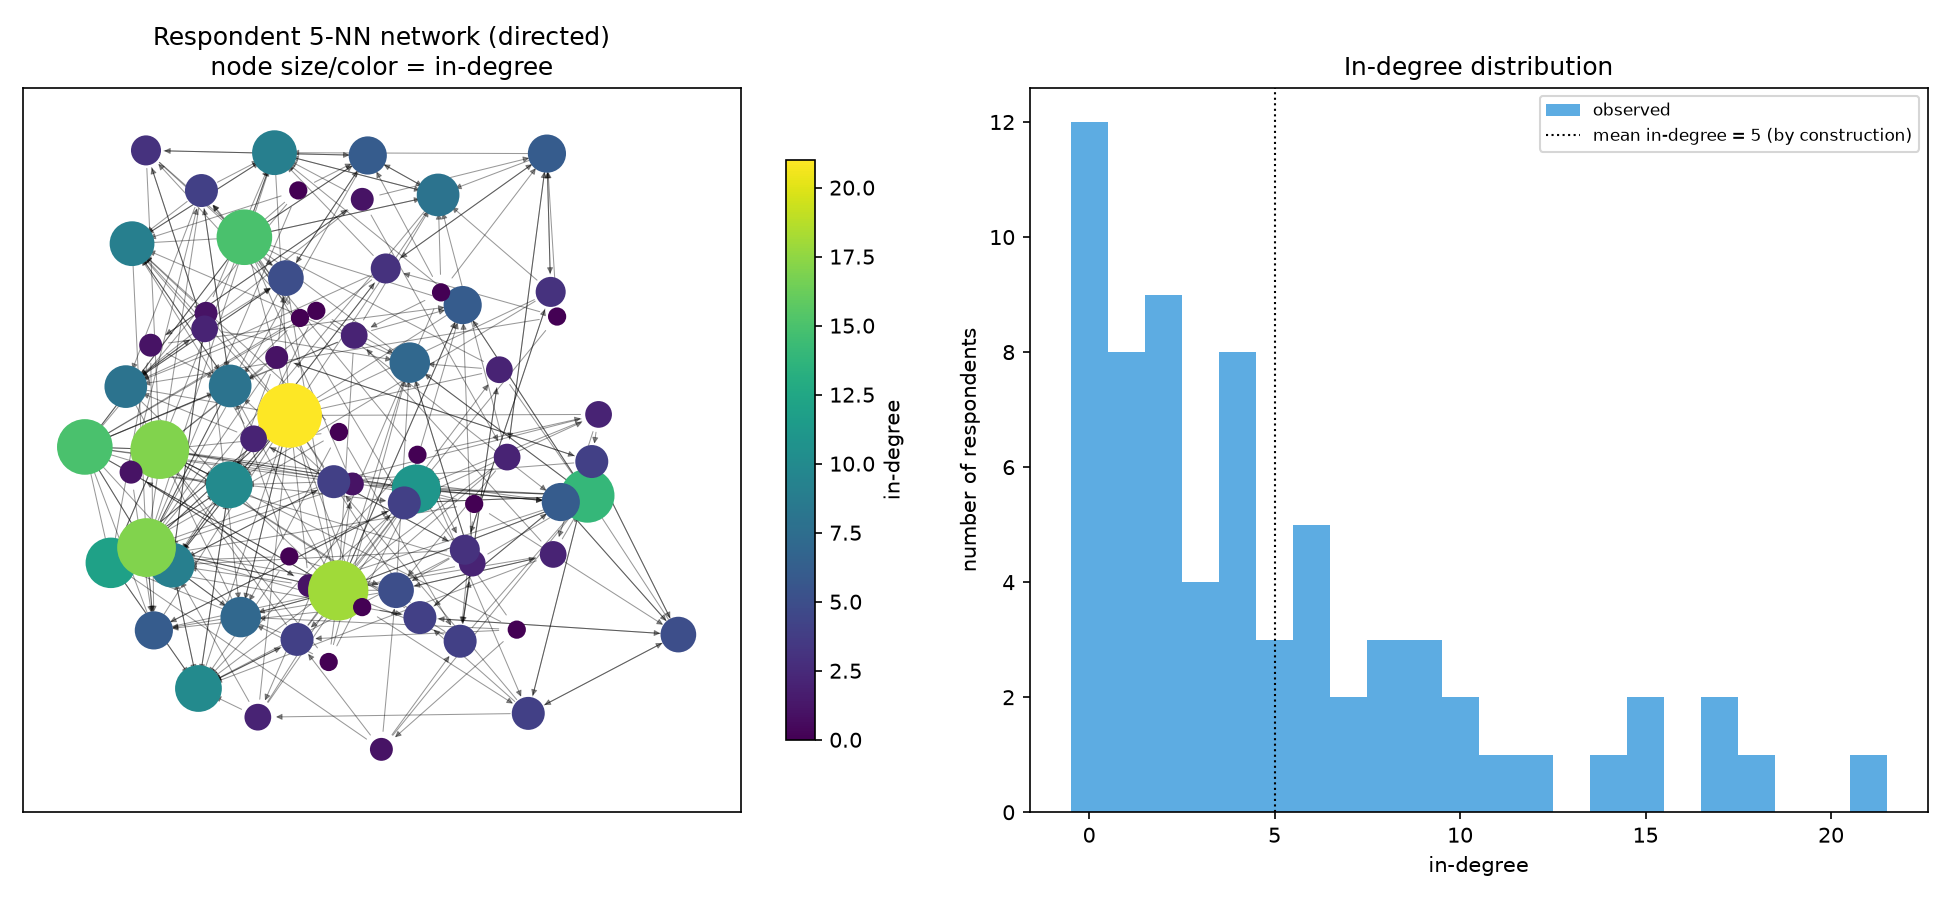
\includegraphics[width=0.8\textwidth]{../outputs/respondent_network.png}

    \caption{Top: network $k$-NN against the global-mean baseline, and the bootstrap behind the
    confidence interval in Table~\ref{tab:headline}. Bottom: the directed 5-NN respondent network and
    its in-degree distribution, a handful of respondents get picked as a neighbor far more often than
    random 5-NN assignment would predict.}
    \label{fig:imputation}
\end{figure}

\begin{figure}[htbp]
    \centering
    \begin{minipage}{0.48\textwidth}
        \centering
        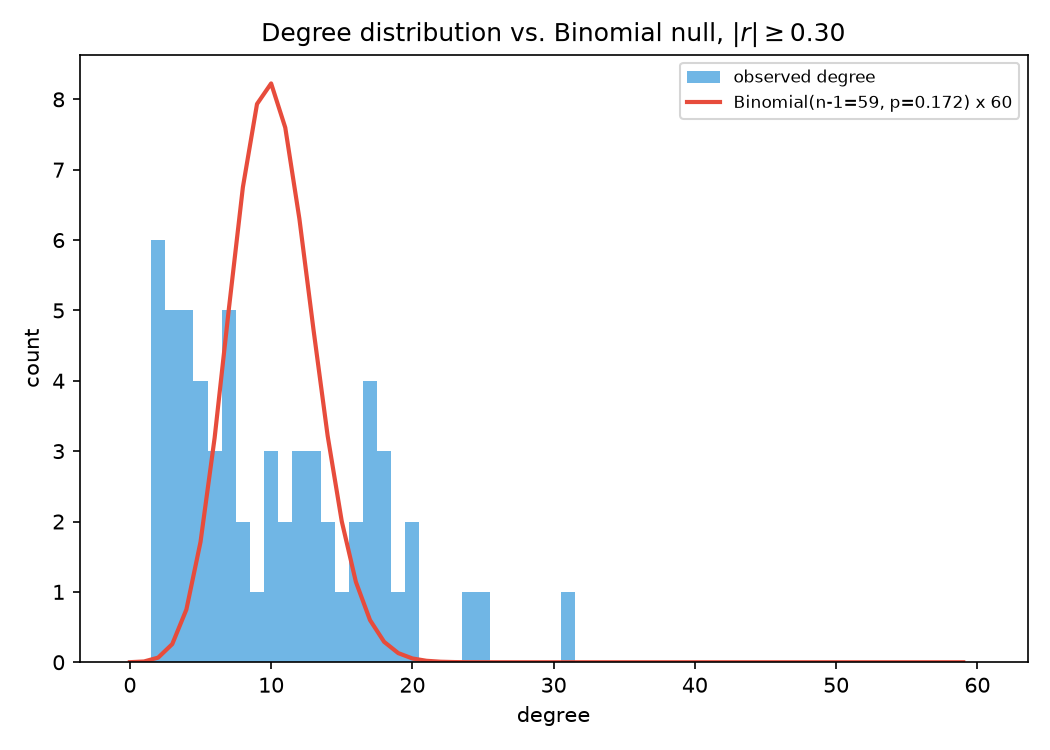
\includegraphics[width=\textwidth]{../outputs/degree_distribution.png}
        \caption{1d: degree distribution at $|r| \geq 0.30$ (blue bars) against a
        Binomial$(59, \hat p)$ null of the same mean (red line). The real distribution is wider.}
        \label{fig:degdist}
    \end{minipage}
    \hfill
    \begin{minipage}{0.48\textwidth}
        \centering
        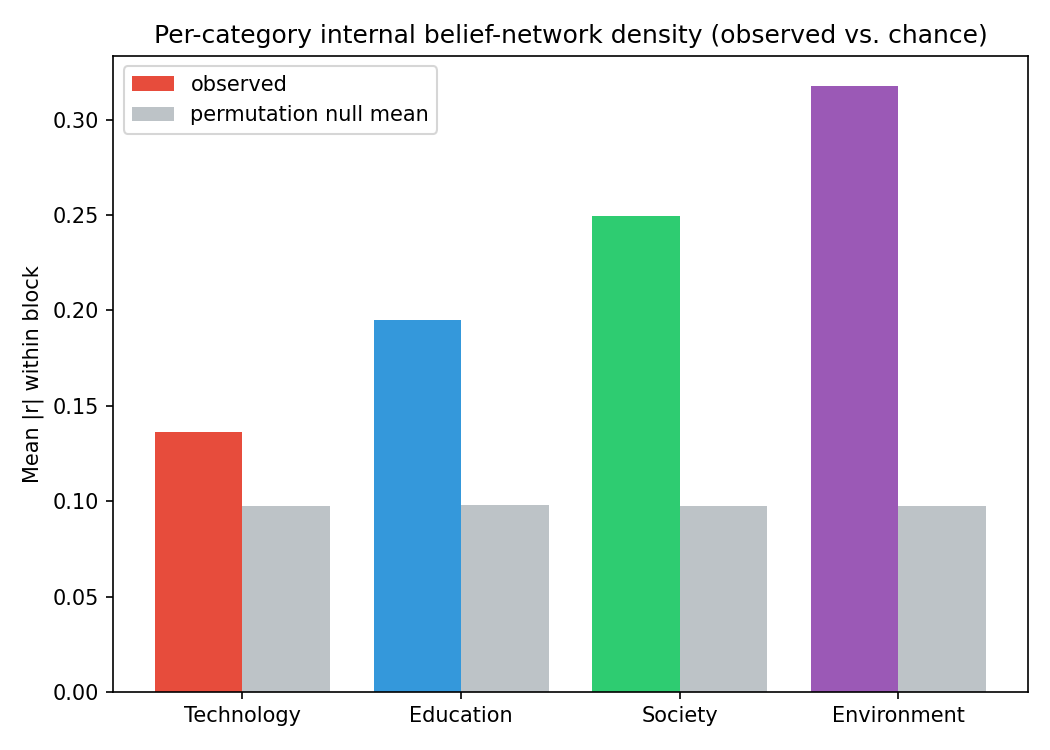
\includegraphics[width=\textwidth]{../outputs/category_density.png}
        \caption{Within-block link density by topic, against each block's own permutation null and
        the closed-form null $\sqrt{2/(\pi(n-1))} \approx 0.098$ (dashed line).}
        \label{fig:density}
    \end{minipage}
\end{figure}

\section{Results and Discussion}

\subsection{Idea: a decoupled Technology cluster, with a caveat}

In the raw data, the centrality ranking puts statements about inclusivity, environmental
accountability, and educational reform at the top, and Technology statements at the bottom almost
across the board (Table~\ref{tab:centrality}). The 22-statement backbone, the core where every member
connects strongly to at least nine others, doesn't contain a single Technology statement. We tested
the Technology-versus-rest centrality gap against 1000 independent reshuffles and never once saw it
matched by chance ($p = 0.0010$), putting the real value about seven standard deviations above the
null mean. PageRank tells the same story as eigenvector centrality (the two rankings correlate at
0.985, so PageRank isn't adding new information here), and betweenness centrality shows the same
pattern: Technology statements bridge the network less than everything else does.

That gap isn't only about Technology as a topic, though. Pearson correlation is sensitive to how
agreeable a respondent is in general, and this class's average per-item agreement ranges from 3.27 to
4.77 out of 5 depending on who you ask. When we rebuild the same graph after subtracting each
respondent's own mean response first, which removes that general agreement level before correlating
items, the centrality gap drops from 0.0668 to 0.0007, basically zero (Figure~\ref{fig:rowcentered}).
That doesn't prove the raw finding is fake. A shared leaning toward pro-social, pro-environment
statements could be a real attitude and not just survey noise, and stripping it out would erase real
signal if that's the case. But we can't tell those two stories apart with this data, so both need
reporting: Technology attitudes are less central in the raw numbers, and most of that gap tracks
general agreement rather than Technology specifically.

\begin{table}[htbp]
    \centering
    \caption{The five most and least central statements by eigenvector centrality. Four of the five
    least central are Technology items.}
    \label{tab:centrality}
    \small
    \begin{tabularx}{\textwidth}{@{}lXr@{}}
        \toprule
        Code & Statement & Centr. \\
        \midrule
        \multicolumn{3}{@{}l}{\textit{Most central (top 5 of 60)}} \\
        S09 & Universities should promote an inclusive environment where different viewpoints can be discussed respectfully. & 0.220 \\
        V07 & Protecting biodiversity is essential for long-term human well-being. & 0.214 \\
        V08 & Universities should adopt environmentally sustainable campus practices even if implementation costs increase. & 0.208 \\
        E07 & Publishing research before graduation should be encouraged, but not mandatory. & 0.191 \\
        S14 & Leaders should prioritize ethical decision-making even when it reduces short-term gains. & 0.187 \\
        \multicolumn{3}{@{}l}{\textit{Least central (bottom 5 of 60)}} \\
        T08 & AI-assisted diagnosis should become routine in healthcare. & 0.022 \\
        T01 & Artificial Intelligence will improve society more than it will create problems. & 0.023 \\
        E06 & Every undergraduate student should participate in at least one research project. & 0.027 \\
        T02 & Generative AI tools should be allowed as learning aids in higher education. & 0.037 \\
        T15 & Society will increasingly depend on AI-assisted decision making. & 0.039 \\
        \bottomrule
    \end{tabularx}
\end{table}

\subsection{Extension 1: structure, disagreement, and threshold sensitivity}

\paragraph{1a, triangle density.} The 647-edge graph has 3049 triangles and a transitivity (clustering
coefficient) of 0.566, against a mean of 1663 triangles and 0.364 transitivity across 200 simulated
Erdos-Renyi graphs of the same size and density ($p = 0.0050$; Figure~\ref{fig:triangle}). So the graph
is more triangle-dense than random chance would give it. That's expected for any correlation graph: if
statement A and B both correlate with C, A and B tend to correlate with each other too, through that
shared variance. It's a sanity check on the graph's structure, not proof of some deeper psychological
consistency mechanism.

\paragraph{1b, the negative-edge subgraph.} Pulling out just the 27 negative edges gives five small
components (sizes 17, 4, 3, 2, 2) with zero triangles (Figure~\ref{fig:negedge}). The biggest one is a
hub-and-spoke shape built around two Education items: E03 ("attendance should be compulsory," degree
9) and E02 ("traditional exams accurately measure knowledge," degree 8). They aren't directly connected
to each other, but they each disagree with a lot of the same surrounding statements. So the
disagreement here is centered on two contested Education items, not on Technology.

\paragraph{1c, threshold sweep.} Sweeping $\tau$ from 0.10 to 0.45 (Table~\ref{tab:sweep}) shows the
null graph's giant component falling apart well before the real one's does: the permutation null
starts shrinking hard around $\tau \approx 0.275$--$0.30$, while the real giant component holds all 60
nodes through $\tau = 0.30$ and only starts losing them after that. Going from $\tau = 0.30$ to
$\tau = 0.35$, 13 statements fall out of the giant component, and 9 of them are Technology. Isolated
nodes show up in much bigger numbers than Erdos-Renyi predicts once the threshold gets strict enough to
break the graph apart (16 observed against 2.3 expected at $\tau = 0.40$). That fits a graph built from
real, uneven correlations rather than uniformly random ones: a tight, well-connected core hangs
together while the weaker, peripheral statements peel off first. The Technology-versus-rest degree gap
stays positive at every single threshold from 0.10 to 0.45, which is why using $\tau = 0.15$ for the
Idea network is a reasonable choice: the Technology finding doesn't depend on this specific number.

\paragraph{1d, structural comparison and degree distribution.} Table~\ref{tab:structural} lines the
graph up against Erdos-Renyi at $\tau = 0.15, 0.20, 0.30$. At every threshold, the observed clustering,
degree variance, and average-neighbor-degree all beat the Erdos-Renyi prediction for a random graph of
the same size and density, most obviously at $\tau = 0.30$ (clustering 0.45 versus a predicted 0.17;
degree variance 45 versus a predicted 8.5). The degree distribution at $\tau = 0.30$ is noticeably
wider than a Binomial$(59, \hat p)$ null with the same mean (Figure~\ref{fig:degdist}). This same
permutation approach also answers why the Idea network uses $|r| \geq 0.15$: roughly 43\% of its 907
edges (about 393) would show up by chance alone, falling to about 28\% at $\tau = 0.20$ (179 of 647)
and about 7\% at $\tau = 0.30$ (23 of 304). We chose 0.15 on purpose, accepting more chance-level edges
in exchange for a graph whose centrality reflects the full correlation structure instead of an
arbitrarily thin slice of it. Part 1c shows this choice doesn't drive the Technology result, it just
controls how much noise rides along with the real signal.

\subsection{Extension 2: a small, borderline predictive effect}

Across all 4080 (respondent, item) cells, with each item's own column dropped from the similarity
calculation before predicting it, the network's $k$-NN prediction gets a mean absolute error of 0.645
against a global-mean baseline of 0.662. That's a small improvement. Because those 4080 cells come from
only 68 people and aren't independent of each other, we used a respondent-level bootstrap instead of a
cell-level test: the 95\% confidence interval for the improvement is $[-0.010, 0.042]$
(Figure~\ref{fig:imputation}), which includes zero. The honest read is a small, borderline effect, not
a strong one.

Looking at the 5-nearest-neighbor structure as a directed graph (Figure~\ref{fig:imputation}, since each
respondent points to five others but isn't necessarily pointed back at by the same five) shows the
in-degree distribution is way more uneven than random assignment would give: standard deviation 5.07
against 2.14 under random assignment, a max in-degree of 21, and 12 respondents nobody picked at all.
In-degree correlates with a respondent's own mean agreement level ($r = 0.43$), people who agree with
more statements on average get picked as a neighbor more often. We don't know why that correlation
holds; it's reported here as a descriptive fact, not an explained one. The six respondents who
abandoned the survey partway through are excluded before this network gets built, so this analysis
says nothing about them.

\subsection{Extension 3: topic-level density, with the same caveat as the Idea}

Every block clears its own permutation null (Table~\ref{tab:headline}), and the empirical null mean of
about 0.098 lines up with the closed-form expectation for two independent 68-observation vectors,
$\sqrt{2/(\pi \cdot 67)} \approx 0.0975$. But the effect sizes are pretty different: Environment's
density above its noise floor (mean $|r| = 0.318$) is roughly 5.7 times Technology's (mean
$|r| = 0.136$). Just like the Idea network, this gap shrinks a lot once each respondent's general
agreement level gets removed first: the row-centered densities converge to roughly 0.12--0.14 across
all four blocks instead of spreading from 0.136 to 0.318 (Figure~\ref{fig:rowcentered}). Technology's
within-block correlations are weakly related to each other compared to Environment's; nothing here
tests for, or backs up, separate sub-views inside any one block.

\subsection{Synthesis}

These four analyses are several views of one correlation structure, not four fully independent
confirmations of each other. The Idea, Extension 1, and Extension 3 all come from the same 60-by-60
item correlation matrix; only Extension 2 uses a genuinely different one, built respondent by
respondent. Even so, read together they point the same way. In the raw data, Technology and AI
statements are less central, they're behind the graph's only real disagreement structure once
Education's hub items are set aside, and they form the least internally correlated topic block. But
the row-centered checks in Sections~4.1 and~4.4 show most of that pattern tracks a general agreement
factor shared across respondents, not something specific to Technology, and Extension 2's corrected
result is small and statistically borderline rather than strong. We didn't test, and this report
doesn't claim, that someone's environmental or ethical positions predict their stance on AI; that
would need its own targeted analysis that this project doesn't include.

\section{Individual Contribution}

\begin{description}[leftmargin=2.2cm, style=nextline]
\item[Abhishek] Built the shared data-loading and permutation-null utility (\texttt{data\_utils.py})
that the rest of the project runs on. Built the statement co-endorsement network and computed its
eigenvector centrality, PageRank, betweenness centrality, and $k$-core backbone. Ran the
centrality-gap significance test at $B=1000$, the PageRank-versus-eigenvector check, the per-block
betweenness stats, and the row-centered robustness check in Section~4.1. Produced the network
visualization in Figure~\ref{fig:network} along with its centrality and significance plots.

\item[Shreyas] Built Extension 1: the Erdos-Renyi triangle-density benchmark,
the negative-edge subgraph analysis, the threshold sweep across edge count, giant-component size,
isolated nodes, and the Technology degree gap, and the structural comparison table with the
degree-distribution check against a Binomial null, including the chance-edge-fraction argument
for why the Idea network uses $|r| \geq 0.15$. Produced Figures~\ref{fig:triangle}, \ref{fig:negedge},
and~\ref{fig:degdist}, and Tables~\ref{tab:sweep} and~\ref{tab:structural}.

\item[Sampath] Built the leave-one-item-out evaluation of the respondent similarity network across all
4080 cells, the respondent-level bootstrap behind its significance test, and the directed-graph
in-degree analysis and visualization of the 5-NN respondent network. Built Extension 3's closed-form
null derivation, its weighted-link-density framing, and its row-centered robustness check, and put
together the combined raw-versus-row-centered comparison figure covering both the Idea and Extension
3 results. Produced Figures~\ref{fig:rowcentered}, \ref{fig:imputation}, and~\ref{fig:density}.
\end{description}

All three of us checked each other's numbers against the shared repository before putting this report
together, and wrote the synthesis in Section~4.5 together.

\end{document}
